\subsection{Statistical analysis of experiment 1}
Here the various statistical methods covered in \cref{subsec:correlation}\cref{subsec:distribution}, will be used to analyses the data. The initial step is to verify if the data is normally distributed as it has a large effect on which statistical methods that can be used to analyze th data. To do this the Shapiro-Wilk test will be used to check if the data is normally distributed. 
The results show that the data for the different DUTs are not all normally distributed, though the vast majority is.
\begin{table}[]
    \begin{tabular}{||c|c|c|c|c|c||}
    \hline
    &\textbf{TestCaseIdle}&\textbf{BinaryTrees}&\textbf{FannkuchRedux}&\textbf{Nbody}&\textbf{Fasta}\\ [0.5ex] \hline\hline
    \textbf{IntelPowerGadget}&0.0004&0.3685&0.0007&0.0&0.0809\\
    \textbf{HardwareMonitor}&0.0&0.0033&0.088&0.0&0.0002\\
    \textbf{E3}&0.9307&0.2229&0.0&0.0966&0.0002\\
    \textbf{RAPL}&0.0152&0.0311&0.0&0.0&0.0007\\ \hline
    \end{tabular}
    \label{tab:NormDistSurfB}
\end{table}
As can be seen in \cref{tab:NormDistSurfB}, the majority are normally distributed if $P = 0.05$, some are not thus we need to use the statistical methods that can handle non-normally distributed data. The first test that will be used in the MannWhitney U test, which is a non-parametric independence test, this allows us to compare the different measurement foreach of the testcases to check if they are are independent from eachother. The expectation are that the $H_0$ can be rejected as Each of the DUT have different energy consumptions, and that each of the instruments measurements are seems to be different.
The results from the FannkuchRedux testcase can be seen below, the maps for the rest can be found in the appendix.
\begin{figure}
  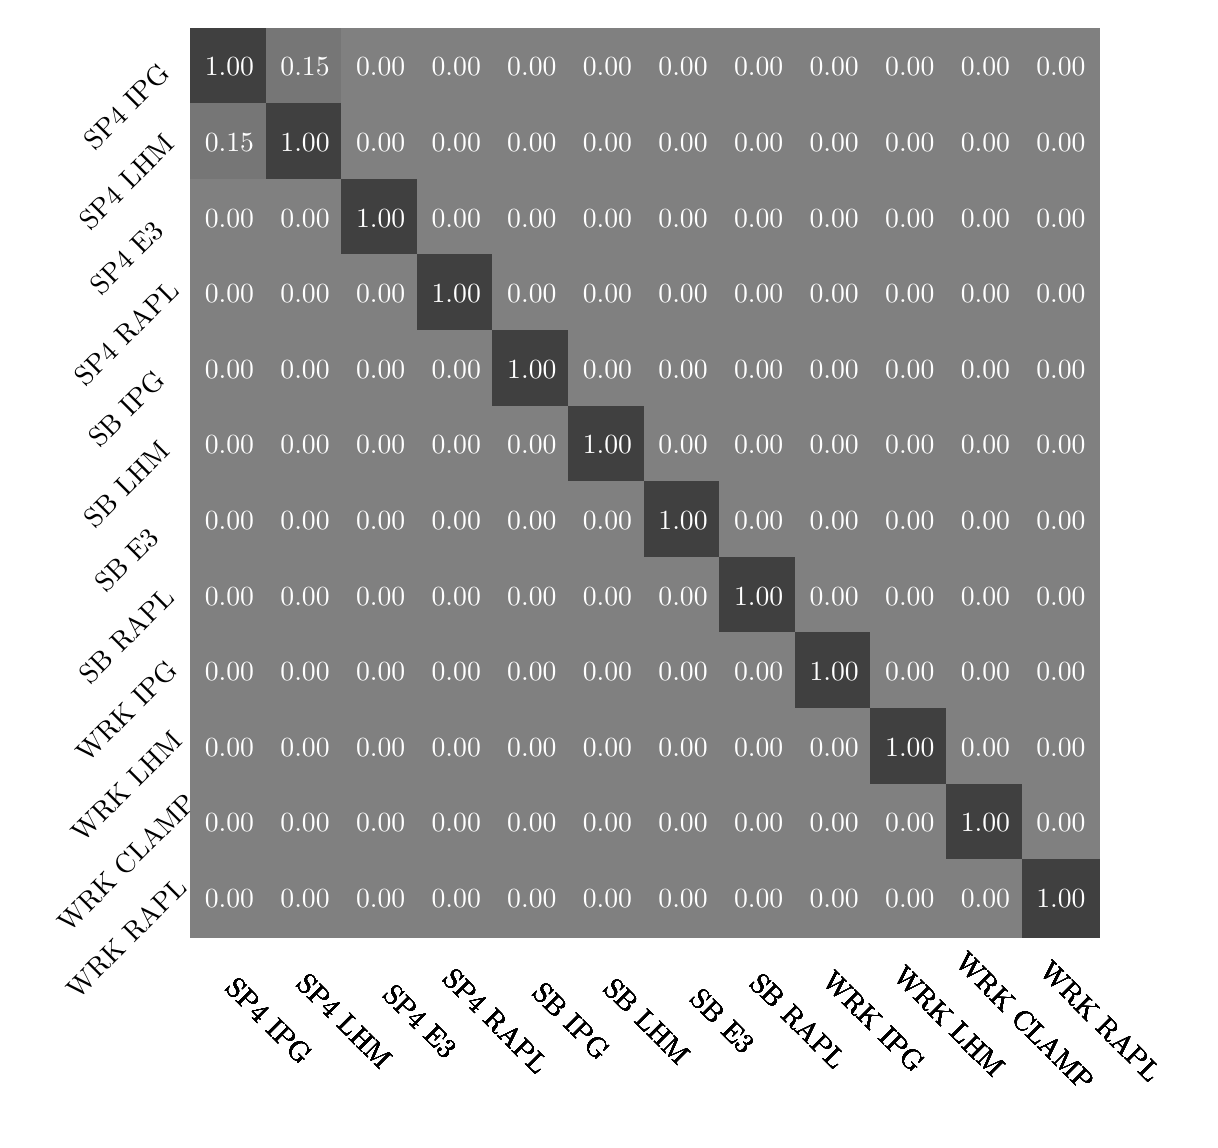
\begin{tikzpicture}[scale=0.6]
    \foreach \y [count=\n] in {{1.00, 0.15, 0.00, 0.00, 0.00, 0.00, 0.00, 0.00, 0.00, 0.00, 0.00, 0.00},{0.15, 1.00, 0.00, 0.00, 0.00, 0.00, 0.00, 0.00, 0.00, 0.00, 0.00, 0.00},{0.00, 0.00, 1.00, 0.00, 0.00, 0.00, 0.00, 0.00, 0.00, 0.00, 0.00, 0.00},{0.00, 0.00, 0.00, 1.00, 0.00, 0.00, 0.00, 0.00, 0.00, 0.00, 0.00, 0.00},{0.00, 0.00, 0.00, 0.00, 1.00, 0.00, 0.00, 0.00, 0.00, 0.00, 0.00, 0.00},{0.00, 0.00, 0.00, 0.00, 0.00, 1.00, 0.00, 0.00, 0.00, 0.00, 0.00, 0.00},{0.00, 0.00, 0.00, 0.00, 0.00, 0.00, 1.00, 0.00, 0.00, 0.00, 0.00, 0.00},{0.00, 0.00, 0.00, 0.00, 0.00, 0.00, 0.00, 1.00, 0.00, 0.00, 0.00, 0.00},{0.00, 0.00, 0.00, 0.00, 0.00, 0.00, 0.00, 0.00, 1.00, 0.00, 0.00, 0.00},{0.00, 0.00, 0.00, 0.00, 0.00, 0.00, 0.00, 0.00, 0.00, 1.00, 0.00, 0.00},{0.00, 0.00, 0.00, 0.00, 0.00, 0.00, 0.00, 0.00, 0.00, 0.00, 1.00, 0.00},{0.00, 0.00, 0.00, 0.00, 0.00, 0.00, 0.00, 0.00, 0.00, 0.00, 0.00, 1.00},} {
    % column labels
    \foreach \a [count=\n] in {SP4 IPG,SP4 LHM,SP4 E3,SP4 RAPL,SB IPG,SB LHM,SB E3,SB RAPL,WRK IPG,WRK LHM,WRK CLAMP,WRK RAPL} {
      \node[minimum size=10mm, xshift=0.5cm, rotate=-45] at (\n*1.6, -21.8) {\a};
    }
    % heatmap tiles
    \foreach \x [count=\m] in \y {
      \pgfmathsetmacro{\xa }{(\x + 1) / 2 * 100}
      \node[fill=darkgray!\xa!lightgray, minimum size=10mm, text=white, font={\normalsize}] at (\m*1.6,-\n*1.6) {\x};
    }
  }
    % row labels
    \foreach \a [count=\i] in {SP4 IPG,SP4 LHM,SP4 E3,SP4 RAPL,SB IPG,SB LHM,SB E3,SB RAPL,WRK IPG,WRK LHM,WRK CLAMP,WRK RAPL} {
      \node[minimum size=10mm, xshift=-0.35cm, yshift=-0.5cm, rotate=45] at (0,-\i*1.6) {\a};
    }
  \end{tikzpicture}
  \caption{Here the results for the FannkuchRedux can be seen}
  \label{tab:HeatFannkuchRedux}
  \end{figure} 
As can be seen in \cref{tab:HeatFannkuchRedux}, the majority of the values are below $p = 0.05$, meaning that we can confidently reject the null hypotheses. The only cases where $H_0$ cannot be rejected is \textbf{SP4 LHM} and \textbf{SP4 IPG}.
Now to take a look at the correlation between the different measurement instruments, kendall tau correlation. To use the kendall tau Correlation, all the test case results for each of the DUTs were appended to eachother and sorted based on the TestCase, an example of which can be seen here.
\input{tabels/experiment_results/exp_one/StatQuest/stats.tex},
In \cref{tab:RainBowGraph} the background of each point represents what test case each point is from these are then used to calculate the Correlation as seen in the following heat maps:
\begin{figure}
\centering
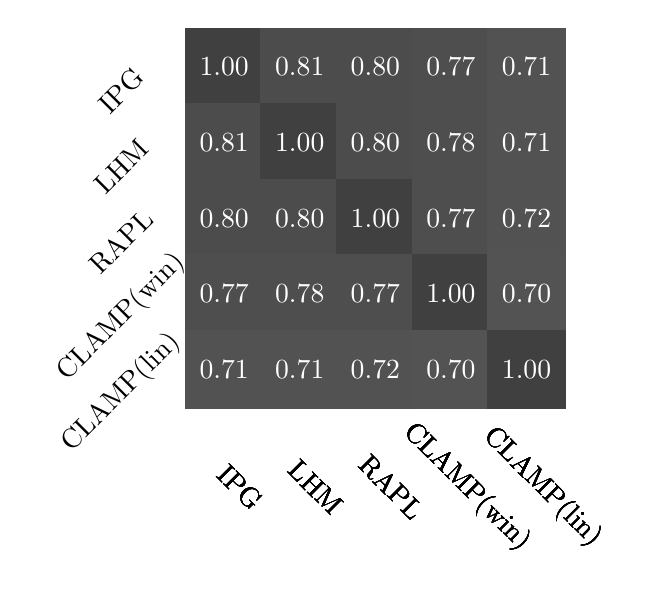
\begin{tikzpicture}[scale=0.6]
  \foreach \y [count=\n] in {{1.00, 0.81, 0.80, 0.77, 0.71},{0.81, 1.00, 0.80, 0.78, 0.71},{0.80, 0.80, 1.00, 0.77, 0.72},{0.77, 0.78, 0.77, 1.00, 0.70},{0.71, 0.71, 0.72, 0.70, 1.00},} {
  % column labels
  \foreach \a [count=\n] in {IPG,LHM,RAPL,CLAMP(win),CLAMP(lin)} {
    \node[minimum size=10mm, xshift=0.2cm, rotate=-45] at (\n*1.6, -10.50) {\a};
  }
  % heatmap tiles
  \foreach \x [count=\m] in \y {
    \pgfmathsetmacro{\xa }{(\x + 1) / 2 * 100}
    \node[fill=darkgray!\xa!lightgray, minimum size=10mm, text=white, font={\normalsize}] at (\m*1.6,-\n*1.6) {\x};
  }
}
  % row labels
  \foreach \a [count=\i] in {IPG,LHM,RAPL,CLAMP(win),CLAMP(lin)} {
    \node[minimum size=10mm, xshift=-0.35cm, yshift=-0.3cm, rotate=45] at (0,-\i*1.6) {\a};
  } 
\end{tikzpicture}
\caption{This heat map represents Correlation coefficients between the different measuring instruments -1 to 1 on the Workstation}
\label{tab:correlationWork}
\end{figure}
\begin{figure}
    \centering
    \begin{subfigure}{.5\textwidth}
      \centering
      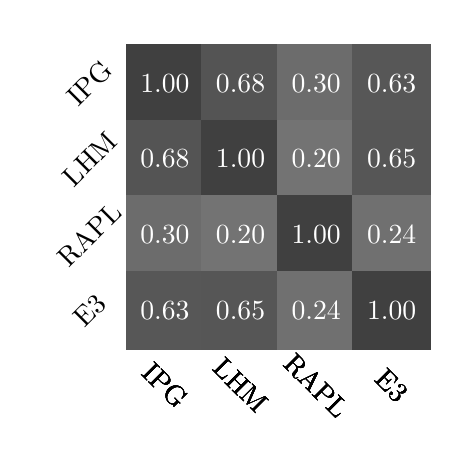
\begin{tikzpicture}[scale=0.6]
        \foreach \y [count=\n] in {{1.00, 0.68, 0.30, 0.63},{0.68, 1.00, 0.20, 0.65},{0.30, 0.20, 1.00, 0.24},{0.63, 0.65, 0.24, 1.00},} {
        % column labels
        \foreach \a [count=\n] in {IPG,LHM,RAPL,E3} {
          \node[minimum size=10mm, xshift=0.0cm, rotate=-45] at (\n*1.6, -8) {\a};
        }
        % heatmap tiles
        \foreach \x [count=\m] in \y {
          \pgfmathsetmacro{\xa }{(\x + 1) / 2 * 100}
          \node[fill=darkgray!\xa!lightgray, minimum size=10mm, text=white, font={\normalsize}] at (\m*1.6,-\n*1.6) {\x};
        }
      }
        % row labels
        \foreach \a [count=\i] in {IPG,LHM,RAPL,E3} {
          \node[minimum size=10mm, xshift=-0.0cm, yshift=-0.0cm, rotate=45] at (0,-\i*1.6) {\a};
        }
      \end{tikzpicture}
    \caption{This heat map represents Correlation coefficients between the different measurement instruments -1 to 1 on the Surface Book}
    \label{tab:correlationSurfP}
    \end{subfigure}%
    \begin{subfigure}{.5\textwidth}
      \centering
      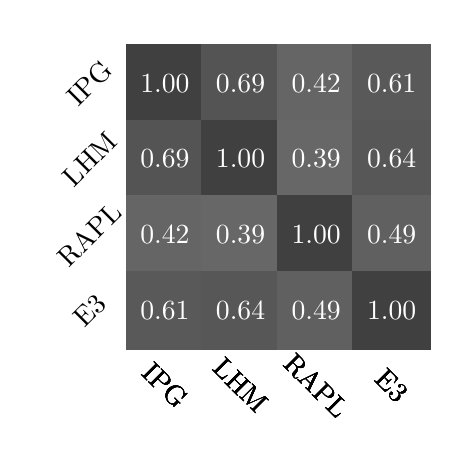
\begin{tikzpicture}[scale=0.6]
        \foreach \y [count=\n] in {{1.00, 0.69, 0.42, 0.61},{0.69, 1.00, 0.39, 0.64},{0.42, 0.39, 1.00, 0.49},{0.61, 0.64, 0.49, 1.00},} {
        % column labels
        \foreach \a [count=\n] in {IPG,LHM,RAPL,E3} {
          \node[minimum size=10mm, xshift=0.0cm, rotate=-45] at (\n*1.6, -8) {\a};
        }
        % heatmap tiles
        \foreach \x [count=\m] in \y {
          \pgfmathsetmacro{\xa }{(\x + 1) / 2 * 100}
          \node[fill=darkgray!\xa!lightgray, minimum size=10mm, text=white, font={\normalsize}] at (\m*1.6,-\n*1.6) {\x};
        }
      }
        % row labels
        \foreach \a [count=\i] in {IPG,LHM,RAPL,E3} {
          \node[minimum size=10mm, xshift=-0.0cm, yshift=-0.0cm, rotate=45] at (0,-\i*1.6) {\a};
        }
      \end{tikzpicture}
    \caption{This heat map represents Correlation coefficients between the different measurement instruments -1 to 1 on the Surface Pro 4}
    \label{tab:HeatFasta}
    \end{subfigure}
\end{figure}
% \begin{figure}
    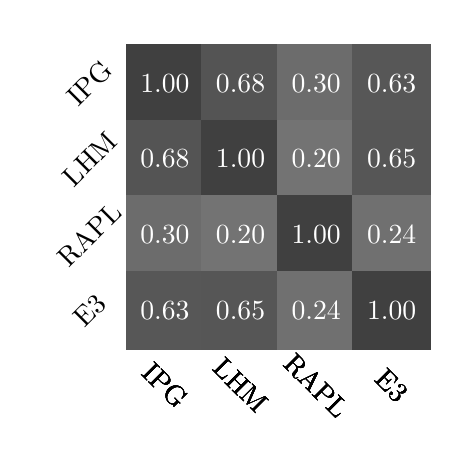
\begin{tikzpicture}[scale=0.6]
        \foreach \y [count=\n] in {{1.00, 0.68, 0.30, 0.63},{0.68, 1.00, 0.20, 0.65},{0.30, 0.20, 1.00, 0.24},{0.63, 0.65, 0.24, 1.00},} {
        % column labels
        \foreach \a [count=\n] in {IPG,LHM,RAPL,E3} {
          \node[minimum size=10mm, xshift=0.0cm, rotate=-45] at (\n*1.6, -8) {\a};
        }
        % heatmap tiles
        \foreach \x [count=\m] in \y {
          \pgfmathsetmacro{\xa }{(\x + 1) / 2 * 100}
          \node[fill=darkgray!\xa!lightgray, minimum size=10mm, text=white, font={\normalsize}] at (\m*1.6,-\n*1.6) {\x};
        }
      }
        % row labels
        \foreach \a [count=\i] in {IPG,LHM,RAPL,E3} {
          \node[minimum size=10mm, xshift=-0.0cm, yshift=-0.0cm, rotate=45] at (0,-\i*1.6) {\a};
        }
      \end{tikzpicture}
    \caption{This heat map represents Correlation coefficients between the different measurement instruments -1 to 1 on the Surface Book}
    \label{tab:correlationSurfP}
\end{figure}
% \begin{figure}
    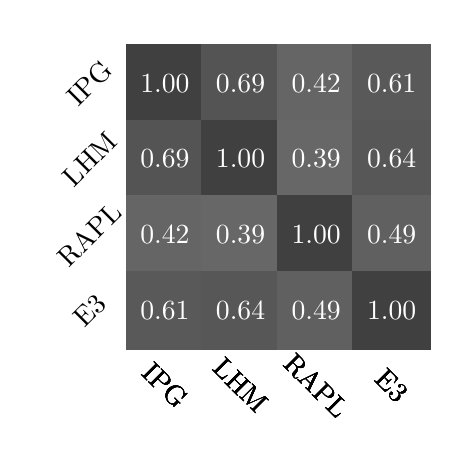
\begin{tikzpicture}[scale=0.6]
        \foreach \y [count=\n] in {{1.00, 0.69, 0.42, 0.61},{0.69, 1.00, 0.39, 0.64},{0.42, 0.39, 1.00, 0.49},{0.61, 0.64, 0.49, 1.00},} {
        % column labels
        \foreach \a [count=\n] in {IPG,LHM,RAPL,E3} {
          \node[minimum size=10mm, xshift=0.0cm, rotate=-45] at (\n*1.6, -8) {\a};
        }
        % heatmap tiles
        \foreach \x [count=\m] in \y {
          \pgfmathsetmacro{\xa }{(\x + 1) / 2 * 100}
          \node[fill=darkgray!\xa!lightgray, minimum size=10mm, text=white, font={\normalsize}] at (\m*1.6,-\n*1.6) {\x};
        }
      }
        % row labels
        \foreach \a [count=\i] in {IPG,LHM,RAPL,E3} {
          \node[minimum size=10mm, xshift=-0.0cm, yshift=-0.0cm, rotate=45] at (0,-\i*1.6) {\a};
        }
      \end{tikzpicture}
    \caption{This heat map represents Correlation coefficients between the different measuring instrument1 on the Surface Pro 4}
    \label{tab:HeatFasta}
\end{figure}
Evaluating the results using the scale presented by Guildford in \cite[219]{guilford1950fundamental} can be used.
\begin{itemize}
    \item $<.20$: Slight; almost negligible relationship
    \item $.20-.40$: Low correlation; definite but small relationship
    \item $.40-.70$: Moderate correlation; substantial relationship
    \item $.70-.90$: High Correlation; marked relationship
    \item $.90-1$: Very high correlation; very dependable relationship
\end{itemize}

using this scale we can evaluate the correlation between the different measuring instruments.
Looking across the different DUTs we can calculate average Correlation between each of the measuring instruments.
$IPG|LHM = (0.68+0.81+0.69)/3 = 0.726$
$IPG|RAPL = (0.30+0.42+0.80)/3 = 0.506$
$LHM|RAPL = (0.80+0.39+0.21)/3 = 0.466$
Since the Clamp is only available on on the workstation it will only be evaluated using the numbers from the workstation.
$IPG|Clamp = (0.77+0.71)/2 = 0.74$
$LHM|Clamp = (0.78+0.71)/2 = 0.745$
$RAPL|Clamp = (0.77+0.72)/2 = 0.745$
A similar situation is present for E3 as it can only be used on the mobile devices.
$IPG|E3 = (0.63+0.61)/2 = 0.62$
$LHM|E3 = (0.65+0.64)/2 = 0.645$
$RAPL|E3 = (0.24+0.49)/2 = 0.365$

Looking at these numbers and evaluating them on the Guildford scale, we can see that IPG|LHM,IPG|Clamp,RAPL|Clamp all are High Correlation and marked relationships, while LHM|RAPL, LHM|RAPL,IPG|E3 and LHM|E3 are Moderate Correlation, substantial relationship. The lowest correlation betweent the measurements was found with RAPL|E3 which are a Low correlation definite but small relationship.

These results seem to indicate that all of the measuring instruments are correlated, which is expected if they actually work, as intended. Another interesting thing to note here is that the correlation between the measurements on the workstation are much higher as opposed to the two laptops. From this it can be seen that many of the measurement instruments seems to measure something close to accurate and this is especially true when looking at the workstation. Another instresting obersvation is that all the measurements are less correlated on the laptops than the Workstation.




